

\def\slidemode{
  \documentclass[fleqn,aspectratio=169]{beamer}
\usepackage{pgfpages}
}
\def\handoutmode{
  \documentclass[handout,fleqn,aspectratio=169]{beamer}
\usepackage{pgfpages}
\pgfpagesuselayout{resize to}[a4paper,landscape,border shrink=5mm]
}


%\def\pdfmode{handoutmode}
\def\pdfmode{slidemode}

\csname\pdfmode\endcsname

\mode<presentation>
{
  \usetheme{default}
  \usecolortheme{default}
  \usefonttheme{default}
  \setbeamertemplate{navigation symbols}{}
  \setbeamertemplate{caption}[numbered]
  \setbeamertemplate{footline}[frame number]  % or "page number"
  \setbeamercolor{frametitle}{fg=white}
  \setbeamercolor{footline}{fg=black}
} 

\usepackage[english]{babel}
%\usepackage[utf8x]{inputenc}
\usepackage{tikz}
\usepackage{courier}
\usepackage{array}
\usepackage{bold-extra}
%\usepackage{minted}
%\usepackage[thicklines]{cancel}
%\usepackage{fancyvrb}
\usepackage{kotex}
\usepackage{paralist}
\usepackage{collectbox}
\usepackage{amsmath}
\usepackage{mathtools}
\usepackage{nccmath}
\usepackage{bm}
\usepackage{booktabs}
\usepackage{tcolorbox}
\usepackage[absolute,overlay]{textpos}

\xdefinecolor{dianablue}{rgb}{0.18,0.24,0.31}
\xdefinecolor{darkblue}{rgb}{0.1,0.1,0.7}
\xdefinecolor{darkgreen}{rgb}{0,0.5,0}
\xdefinecolor{darkgrey}{rgb}{0.35,0.35,0.35}
\xdefinecolor{darkorange}{rgb}{0.8,0.5,0}
\xdefinecolor{darkred}{rgb}{0.7,0,0}
\definecolor{darkgreen}{rgb}{0,0.6,0}
\definecolor{mauve}{rgb}{0.58,0,0.82}



\title[]{Lecture 2: Conditioning, Bayes' Rule, and Independence }
\author{Yi, Yung (이융)}
\institute{EE210: Probability and Introductory Random Processes\\ KAIST EE}
\date{\today}

%%%%%%%%%%%% real, integer notation
\newcommand{\real}{{\mathbb R}}
\newcommand{\integer}{{\mathbb Z}}

%%% set, vector, matrix
\newcommand{\set}[1]{\ensuremath{\mathcal #1}}
\renewcommand{\vec}[1]{\bm{#1}}
\newcommand{\mat}[1]{\bm{#1}}


%%% big parenthesis
\def\Bl{\Bigl}
\def\Br{\Bigr}
\def\lf{\left}
\def\ri{\right}


%%% floor notations
\newcommand{\lfl}{{\lfloor}}
\newcommand{\rfl}{{\rfloor}}
\newcommand{\floor}[1]{{\lfloor #1 \rfloor}}

%%% gradient
\newcommand{\grad}[1]{\nabla #1}

%%% definition
\newcommand{\eqdef}{\ensuremath{\triangleq}}
%%% imply
\newcommand{\imp}{\Longrightarrow}



\newcommand{\separator}{
%  \begin{center}
    \par\noindent\rule{\columnwidth}{0.3mm}
%  \end{center}
}

\newcommand{\mynote}[1]{{\it \color{red} [#1]}}







%%% equation alignment
\newcommand{\aleq}[1]{\begin{align*}#1\end{align*}}

%%%%%%%%%%%%%%%% colored emphasized font, blanked words

\newcommand{\empr}[1]{{\color{red}\emph{#1}}}
\newcommand{\empb}[1]{{\color{blue}\emph{#1}}}

%normal colored text
\newcommand{\redf}[1]{{\color{red} #1}}
\newcommand{\yellowf}[1]{{\color{yellow} #1}}
\newcommand{\bluef}[1]{{\color{blue} #1}}
\newcommand{\grayf}[1]{{\color{gray} #1}}
\newcommand{\magenf}[1]{{\color{magenta} #1}}
\newcommand{\greenf}[1]{{\color{green} #1}}
\newcommand{\cyanf}[1]{{\color{cyan} #1}}
\newcommand{\orangef}[1]{{\color{orange} #1}}


\newcommand{\blk}[1]{\underline{\mbox{\hspace{#1}}}}


\newcommand{\redblk}[1]{\framebox{\color{red} #1}}
\newcommand{\redblank}[2]{\framebox{\onslide<#1->{\color{red} #2}}}
\newcommand{\blueblk}[1]{\framebox{\color{blue} #1}}
\newcommand{\blueblank}[2]{\framebox{\onslide<#1->{\color{blue} #2}}}



\makeatletter
\newcommand{\mybox}{%
    \collectbox{%
        \setlength{\fboxsep}{1pt}%
        \fbox{\BOXCONTENT}%
    }%
}
\makeatother

\makeatletter
\newcommand{\lecturemark}{%
    \collectbox{%
        \setlength{\fboxsep}{1pt}%
        \fcolorbox{red}{yellow}{\BOXCONTENT}%
    }%
}
\makeatother

\usepackage{tcolorbox}
\newcommand{\mycolorbox}[1]{
\begin{tcolorbox}[colback=red!5!white,colframe=red!75!black]
#1
\end{tcolorbox}
}

%%%% figure inclusion
\newcommand{\mypic}[2]{
\begin{center}
\includegraphics[width=#1\textwidth]{#2}
\end{center}
}

\newcommand{\myinlinepic}[2]{
\makebox[0cm][r]{\raisebox{-4ex}{\includegraphics[height=#1]{#2}}}
}


%%%% itemized and enumerated list
\newcommand{\bci}{\begin{compactitem}}
\newcommand{\eci}{\end{compactitem}}
\newcommand{\bce}{\begin{compactenum}}
\newcommand{\ece}{\end{compactenum}}


%%%% making 0.5/0.5 two columns
%%%% how to use: first number: length of separation bar
% \mytwocols{0.6}
% {
% contents in the left column
% }
% {
% contents in the right column
% }
%%%%
\newcommand{\mytwocols}[3]{
\begin{columns}[T] \column{.499\textwidth} #2 \column{.001\textwidth} \rule{.3mm}{{#1}\textheight} \column{.499\textwidth} #3 \end{columns}}

\newcommand{\mythreecols}[4]{
\begin{columns}[T] \column{.31\textwidth} #2 \column{.001\textwidth} \rule{.3mm}{{#1}\textheight} \column{.31\textwidth} #3 \column{.001\textwidth} \rule{.3mm}{{#1}\textheight} \column{.31\textwidth} #4  \end{columns}}

\newcommand{\mysmalltwocols}[3]{
\begin{columns}[T] \column{.4\textwidth} #2 \column{.001\textwidth} \rule{.3mm}{{#1}\textheight} \column{.4\textwidth} #3 \end{columns}}

%%%% making two columns with customized ratios
%%%% how to use:
%first parameter: length of separation bar
%second parameter: ratio of left column
%third parameter: ratio of right column
% \mytwocols{0.6}{0.7}{0.29}
% {
% contents in the left column
% }
% {
% contents in the right column
% }
%%%%
\newcommand{\myvartwocols}[5]{
\begin{columns}[T] \column{#2\textwidth} {#4} \column{.01\textwidth} \rule{.3mm}{{#1}\textheight} \column{#3\textwidth} {#5} \end{columns}}

%%% making my block in beamer
%%% first parameter: title of block
%%% second parameter: contents of block
\newcommand{\myblock}[2]{
\begin{block}{#1} {#2}  \end{block}}

%%% independence notation
\newcommand{\indep}{\perp \!\!\! \perp}

%%%% probability with different shapes (parenthesis or bracket) and different sizes
%%% `i' enables us to insert the subscript to the probability
\newcommand{\bprob}[1]{\mathbb{P}\Bl[ #1 \Br]}
\newcommand{\prob}[1]{\mathbb{P}[ #1 ]}
\newcommand{\cbprob}[1]{\mathbb{P}\Bl( #1 \Br)}
\newcommand{\cprob}[1]{\mathbb{P}( #1 )}
\newcommand{\probi}[2]{\mathbb{P}_{#1}[ #2 ]}
\newcommand{\bprobi}[2]{\mathbb{P}_{#1}\Bl[ #2 \Br]}
\newcommand{\cprobi}[2]{\mathbb{P}_{#1}( #2 )}
\newcommand{\cbprobi}[2]{\mathbb{P}_{#1}\Bl( #2 \Br)}

%%%% expectation with different shapes (parenthesis or bracket) and different sizes
%%% `i' enables us to insert the subscript to the expectation
\newcommand{\expect}[1]{\mathbb{E}[ #1 ]}
\newcommand{\cexpect}[1]{\mathbb{E}( #1 )}
\newcommand{\bexpect}[1]{\mathbb{E}\Bl[ #1 \Br]}
\newcommand{\cbexpect}[1]{\mathbb{E}\Bl( #1 \Br)}
\newcommand{\bbexpect}[1]{\mathbb{E}\lf[ #1 \ri]}
\newcommand{\expecti}[2]{\mathbb{E}_{#1}[ #2 ]}
\newcommand{\bexpecti}[2]{\mathbb{E}_{#1}\Bl[ #2 \Br]}
\newcommand{\bbexpecti}[2]{\mathbb{E}_{#1}\lf[ #2 \ri]}

%%%% variance
\newcommand{\var}[1]{\text{var}[ #1 ]}
\newcommand{\bvar}[1]{\text{var}\Bl[ #1 \Br]}
\newcommand{\cvar}[1]{\text{var}( #1 )}
\newcommand{\cbvar}[1]{\text{var}\Bl( #1 \Br)}

%%%% covariance
\newcommand{\cov}[1]{\text{cov}( #1 )}
\newcommand{\bcov}[1]{\text{cov}\Bl( #1 \Br)}

%%% Popular pmf, pdf notation to avoid long typing
\newcommand{\px}{\ensuremath{p_X(x)}}
\newcommand{\py}{\ensuremath{p_Y(y)}}
\newcommand{\pz}{\ensuremath{p_Z(z)}}
\newcommand{\pxA}{\ensuremath{p_{X|A}(x)}}
\newcommand{\pyA}{\ensuremath{p_{Y|A}(y)}}
\newcommand{\pzA}{\ensuremath{p_{Z|A}(z)}}
\newcommand{\pxy}{\ensuremath{p_{X,Y}(x,y)}}
\newcommand{\pxcy}{\ensuremath{p_{X|Y}(x|y)}}
\newcommand{\pycx}{\ensuremath{p_{Y|X}(y|x)}}

\newcommand{\fx}{\ensuremath{f_X(x)}}
\newcommand{\Fx}{\ensuremath{F_X(x)}}
\newcommand{\fy}{\ensuremath{f_Y(y)}}
\newcommand{\Fy}{\ensuremath{F_Y(y)}}
\newcommand{\fz}{\ensuremath{f_Z(z)}}
\newcommand{\Fz}{\ensuremath{F_Z(z)}}
\newcommand{\fxA}{\ensuremath{f_{X|A}(x)}}
\newcommand{\fyA}{\ensuremath{f_{Y|A}(y)}}
\newcommand{\fzA}{\ensuremath{f_{Z|A}(z)}}
\newcommand{\fxy}{\ensuremath{f_{X,Y}(x,y)}}
\newcommand{\Fxy}{\ensuremath{F_{X,Y}(x,y)}}
\newcommand{\fxcy}{\ensuremath{f_{X|Y}(x|y)}}
\newcommand{\fycx}{\ensuremath{f_{Y|X}(y|x)}}

\newcommand{\fth}{\ensuremath{f_\Theta(\theta)}}
\newcommand{\fxcth}{\ensuremath{f_{X|\Theta}(x|\theta)}}
\newcommand{\fthcx}{\ensuremath{f_{\Theta|X}(\theta|x)}}

\newcommand{\pkcth}{\ensuremath{p_{X|\Theta}(k|\theta)}}
\newcommand{\fthck}{\ensuremath{f_{\Theta|X}(\theta|k)}}


%%%% indicator
\newcommand{\indi}[1]{\mathbf{1}_{ #1 }}

%%%% exponential rv.
\newcommand{\elambdax}{\ensuremath{e^{-\lambda x}}}

%%%% normal  rv.
\newcommand{\stdnormal}{\ensuremath{\frac{1}{\sqrt{2\pi}} e^{-x^2/2}}}
\newcommand{\gennormal}{\ensuremath{\frac{1}{\sigma\sqrt{2\pi}} e^{-(x-\mu)^2/2}}}

%%%%%% estimator, estimate
\newcommand{\hth}{\ensuremath{\hat{\theta}}}
\newcommand{\hTH}{\ensuremath{\hat{\Theta}}}
\newcommand{\MAP}{\ensuremath{\text{MAP}}}
\newcommand{\LMS}{\ensuremath{\text{LMS}}}
\newcommand{\LLMS}{\ensuremath{\text{L}}}
\newcommand{\ML}{\ensuremath{\text{ML}}}

%%%% colored text
\newcommand{\red}[1]{\color{red}#1}
\newcommand{\cyan}[1]{\color{cyan}#1}
\newcommand{\magenta}[1]{\color{magenta}#1}
\newcommand{\blue}[1]{\color{blue}#1}
\newcommand{\green}[1]{\color{green}#1}
\newcommand{\white}[1]{\color{white}#1}

\newcommand{\defi}{{\color{red} Definition.} }
\newcommand{\proff}{{\color{red} Proof.} }
\newcommand{\exam}{{\color{red} Example.} }
\newcommand{\question}{{\color{red} Question.} }
\newcommand{\thm}{{\color{red} Theorem.} }
\newcommand{\background}{{\color{red} Background.} }
\newcommand{\msg}{{\color{red} Message.} }

\newcommand{\bern}[1]{\ensuremath{\text{Bern}(#1)} }
\newcommand{\bp}[1]{\ensuremath{\text{BP}(#1)} }
\newcommand{\poisson}[1]{\ensuremath{\text{Poisson}(#1)} }
\newcommand{\pp}[1]{\ensuremath{\text{PP}(#1)} }


%%%%%%%%%%%%%%%%%%%%%%% old macros that you can ignore %%%%%%%%%%%%%%%%%%%%%%%%

% \def\un{\underline}
% \def\ov{\overline}


% \newcommand{\beq}{\begin{eqnarray*}}
% \newcommand{\eeq}{\end{eqnarray*}}
% \newcommand{\beqn}{\begin{eqnarray}}
% \newcommand{\eeqn}{\end{eqnarray}}
% \newcommand{\bemn}{\begin{multiline}}
% \newcommand{\eemn}{\end{multiline}}
% \newcommand{\beal}{\begin{align}}
% \newcommand{\eeal}{\end{align}}
% \newcommand{\beas}{\begin{align*}}
% \newcommand{\eeas}{\end{align*}}



% \newcommand{\bd}{\begin{displaymath}}
% \newcommand{\ed}{\end{displaymath}}
% \newcommand{\bee}{\begin{equation}}
% \newcommand{\eee}{\end{equation}}


% \newcommand{\vs}{\vspace{0.2in}}
% \newcommand{\hs}{\hspace{0.5in}}
% \newcommand{\el}{\end{flushleft}}
% \newcommand{\bl}{\begin{flushleft}}
% \newcommand{\bc}{\begin{center}}
% \newcommand{\ec}{\end{center}}
% \newcommand{\remove}[1]{}

% \newtheorem{theorem}{Theorem}
% \newtheorem{corollary}{Corollary}
% \newtheorem{prop}{Proposition}
% \newtheorem{lemma}{Lemma}
% \newtheorem{defi}{Definition}
% \newtheorem{assum}{Assumption}
% \newtheorem{example}{Example}
% \newtheorem{property}{Property}
% \newtheorem{remark}{Remark}

% \newcommand{\separator}{
%   \begin{center}
%     \rule{\columnwidth}{0.3mm}
%   \end{center}
% }

% \newenvironment{separation}
% { \vspace{-0.3cm}
%   \separator
%   \vspace{-0.25cm}
% }
% {
%   \vspace{-0.5cm}
%   \separator
%   \vspace{-0.15cm}
% }

% \def\A{\mathcal A}
% \def\oA{\overline{\mathcal A}}
% \def\S{\mathcal S}
% \def\D{\mathcal D}
% \def\eff{{\rm Eff}}
% \def\bD{\bm{D}}
% \def\cU{{\cal U}}
% \def\bbs{{\mathbb{s}}}
% \def\bbS{{\mathbb{S} }}
% \def\cM{{\cal M}}
% \def\bV{{\bm{V}}}
% \def\cH{{\cal H}}
% \def\ch{{\cal h}}
% \def\cR{{\cal R}}
% \def\cV{{\cal V}}
% \def\cA{{\cal A}}
% \def\cX{{\cal X}}
% \def\cN{{\cal N}}
% \def\cJ{{\cal J}}
% \def\cK{{\cal K}}
% \def\cL{{\cal L}}
% \def\cI{{\cal I}}
% \def\cY{{\cal Y}}
% \def\cZ{{\cal Z}}
% \def\cC{{\cal C}}
% \def\cR{{\cal R}}
% \def\id{{\rm Id}}
% \def\st{{\rm st}}
% \def\cF{{\cal F}}
% \def\bz{{\bm z}}
% \def\cG{{\cal G}}
% \def\N{\mathbb{N}}
% \def\bbh{\mathbb{h}}
% \def\bbH{\mathbb{H}}
% \def\bbi{\mathbb{i}}
% \def\bbI{\mathbb{I}}
% \def\R{\mathbb{R}}
% \def\bbR{\mathbb{R}}
% \def\bbr{\mathbb{r}}
% \def\cB{{\cal B}}
% \def\cP{{\cal P}}
% \def\cS{{\cal S}}
% \def\bW{{\bm W}}
% \def\bc{{\bm c}}

% %\def\and{\quad\mbox{and}\quad}
% \def\ind{{\bf 1}}


% \def\bmg{{\bm{\gamma}}}
% \def\bmr{{\bm{\rho}}}
% \def\bmq{{\bm{q}}}
% \def\bmt{{\bm{\tau}}}
% \def\bmn{{\bm{n}}}
% \def\bmcapn{{\bm{N}}}
% \def\bmrho{{\bm{\rho}}}

% \def\igam{\underline{\gamma}(\lambda)}
% \def\sgam{\overline{\gamma}(\lambda)}
% \def\ovt{\overline{\theta}}
% \def\ovT{\overline{\Theta}}
% \def\PP{{\mathrm P}}
% \def\EE{{\mathrm E}}
% \def\iskip{{\vskip -0.4cm}}
% \def\siskip{{\vskip -0.2cm}}

% \def\bp{\noindent{\it Proof.}\ }
% \def\ep{\hfill $\Box$}



\begin{document}

%itemshape
\setbeamertemplate{itemize item}{\scriptsize\raise1.25pt\hbox{\donotcoloroutermaths$\bullet$}}
\setbeamertemplate{itemize subitem}{\tiny\raise1.5pt\hbox{\donotcoloroutermaths$\circ$}}
\setbeamertemplate{itemize subsubitem}{\tiny\raise1.5pt\hbox{\donotcoloroutermaths$\blacktriangleright$}}
%default value for spacing
\plitemsep 0.1in
\pltopsep 0.03in
\setlength{\parskip}{0.15in}
%\setlength{\parindent}{-0.5in}
\setlength{\abovedisplayskip}{0.07in}
\setlength{\mathindent}{0cm}
\setbeamertemplate{frametitle continuation}{[\insertcontinuationcount]}

\setlength{\leftmargini}{0.5cm}
\setlength{\leftmarginii}{0.5cm}

\setlength{\fboxrule}{0.05pt}
\setlength{\fboxsep}{5pt}

\begin{frame}
  \titlepage
\end{frame}


%%%%%%%%%%%%%%%%%%%%%%%%%%%%%%%%%%%%%%%%%%%%%%%%%%%%%%
\begin{frame}{Roadmap}

\plitemsep 0.2in

\bce[(1)]
\item Conditional Probability
\bci
\item How should I change my belief about event $A$, if I come to know that event $B$ occurs?
\eci


\item Bayes' Rule and Bayesian Inference
\bci
\item prob. of $A$ given that $B$ occurs vs. prob. of $B$ given that $A$ occurs

\eci


\item Independence, Conditional Independence
\bci
\item Can I ignore my knowledge about event $B$, when I consider event $A$? 
\eci

\ece
\end{frame}

%%%%%%%%%%%%%%%%%%%%%%%%%%%%%%%%%%%%%%%%%%%%%%%%%%%%%%
\section{L2(1)}
\begin{frame}{Roadmap}



\bce[(1)]
\item \redf{Conditional Probability}

\item \grayf{Bayes' Rule and Bayesian Inference

\item Independence, Conditional Independence}

\ece
\end{frame}

% START START START START START START START START START START START START START

%%%%%%%%%%%%%%%%%%%%%%%%%%%%%%%%%%%%%%%%%%%%%%%%%%%%%%
\begin{frame}{Motivating Example}

\plitemsep 0.1in
\bci 

\item<1-> Pick a person $a$ at random

- event $A$: $a$'s age $\leq$ 20

- event $B$: $a$ is married


\item<2-> \redf{(Q1)} What is the probability of $A$?

\item<2-> \redf{(Q2)} What is the probability of $A$, if I know that that $B$ is true?

\item<3-> Clearly, the above two should be different. I will assign \bluef{lower} probability for \redf{(Q2)}.

\item<4-> \redf{Question:} How should I change my belief, given some additional information?

\item<5-> Need to build up a new theoretical concept, which we call \redblank{6}{conditional probability}.

\eci 

\end{frame}

%%%%%%%%%%%%%%%%%%%%%%%%%%%%%%%%%%%%%%%%%%%%%%%%%%%%%%
\begin{frame}{Conditional Probability: Notation}

%\plitemsep 0.1in
\bci

\item<1-> First, let's choose the notation. "Probability of $A,$ given $B$ occurs". What do you recommend?

\onslide<2->{
$$
{\mathbb P}(A)(B), \quad {\mathbb P}_{B}(A), \quad {\mathbb P}^{B}(A), \quad (B){\mathbb P}(A), \ldots
$$
}
\item<3-> People's choice is ... \redblank{4}{$\cprob{A \mid  B}$}

\item<5-> From now on, given $B$, $\cprob{\cdot | B}$ should be a new \redblank{6}{probability law.}
\bci
\item<6-> \bluef{Three axioms}\footnote{Non-negativity, Normalization, Countable Additivity}  should be satisfied.
\eci

\eci 

\end{frame}

%%%%%%%%%%%%%%%%%%%%%%%%%%%%%%%%%%%%%%%%%%%%%%%%%%%%%%
\begin{frame}{Conditional Probability: Definition (1)}

\plitemsep 0.1in
\bci 

\item<1-> Second, let's define $\cprob{A | B}$. What would it be a good definition?

\item<2-> Probability of $A$ given $B$ $\rightarrow$ both $A$ and $B$ occur. Then, what about this?
$$
\cprob{A \mid B} \eqdef \redf{\cprob{A \cap B}}
$$

\item<3-> Is it good or bad? Why good? Why bad?

\item<4-> Reasons why it is bad: 

\bci
\item $\cprob{\cdot | B}$ should be a new probability law (thus, three axioms)
\eci


\medskip

\onslide<5->{
\bci
  \item $\cprob{\Omega | B}=1$?

  \item $\cprob{B | B}=1$ from our common sense. 
  \item True?
\eci
}
% \item How to fix this? Normalization! 
% \beq
% \cprob{A | B} &\eqdef& \frac{\cprob{A \cap B}}{\cprob{B}}, \quad for \quad \cprob{B} >0.
% \eeq


\eci 

\end{frame}

%%%%%%%%%%%%%%%%%%%%%%%%%%%%%%%%%%%%%%%%%%%%%%%%%%%%%%
\begin{frame}{Conditional Probability: Definition (2)}

\plitemsep 0.1in
\bci 

\item<1-> How to fix this? \redblank{2}{Normalization} 
\onslide<3->{
\mycolorbox{
$$
\cprob{A \mid B} \eqdef \frac{\cprob{A \cap B}}{\orangef{\cprob{B}}}, \quad \text{for} \quad \cprob{B} >0.
$$
}

\bci
\item  Note that this is a \bluef{definition,} not a \bluef{theorem.}} 
\item So, it's not about right or wrong. It's about how happy we are about this definition. 
\eci

\item<4-> All properties of the law $\cprob{\cdot}$ is applied to the conditional law $\cprob{\cdot | B}.$ 
\bci
\item<5-> \bluef{Non-negativity.} $\cprob{A | B}$ for any event $A$?
\item<6-> \bluef{Finite additivity} and thus \bluef{countable additivity.} For any two disjoint  $A$ and $C$,
\aleq{
\cprob{A \cup C \redf{\mid B}} = 
\onslide<7->{\frac{\bprob{(A \cup C) \cap B}}{\cprob{B}} = \frac{\bprob{(A \cap B) \cup (C \cap B)}}{\cprob{B}} }
= \cprob{A \redf{\mid B}} + \cprob{C \redf{\mid B}}
}
\eci

% \item<4-> For example, finite additivity. For two disjoint events $A$ and $C$, 

% \item<5-> Can easily check other axioms for a new probability law $\cprob{\cdot | B}$: Nonnegativity and countable additivity.  


\eci 

\end{frame}



%%%%%%%%%%%%%%%%%%%%%%%%%%%%%%%%%%%%%%%%%%%%%%%%%%%%%%
\section{L2(2)}
\begin{frame}{Roadmap}

\bce[(1)]
\item \grayf{Conditional Probability}

\item \redf{Bayes' Rule and Bayesian Inference}

\item \grayf{Independence, Conditional Independence}

\ece
\end{frame}


%%%%%%%%%%%%%%%%%%%%%%%%%%%%%%%%%%%%%%%%%%%%%%%%%%%%%%
\begin{frame}{}
\vspace{2cm}
\LARGE From now on, using the theory of probability and conditional probability constructed so far, we will develop interesting properties and theorems which are very useful to answer some exciting questions. 

\medskip

\LARGE That is \empr{Bayes' Rule} to make some \empb{inference (추론).}

\end{frame}

%%%%%%%%%%%%%%%%%%%%%%%%%%%%%%%%%%%%%%%%%%%%%%%%%%%%%%
\begin{frame}{Example: (Bayesian) Inference}

\mytwocols{0.5}
{
\plitemsep 0.1in
\bci 

\item<2-> $A_1$: Happy (:-)), $A_2$: Sad (:-()
\item<2-> $B$: Shout

\item<4-> Assume that somebody gives you the following information:
$$
\cprob{A_1}, \quad \cprob{A_2}, \quad \cprob{B | A_1}, \quad\cprob{B | A_2}.
$$

\item<6-> \redf{Question:} $\cprob{A_1 | B}$ and $\cprob{A_2 | B}$?
\eci 
}
{
\plitemsep 0.1in
\bci 

\item<3-> $A_i$: state/cause/original value
\item<3-> $B$: result/resulting action/noisy measurement

\item<5-> In reality, $\cprob{A_i}$ and $\cprob{B | A_i}$ (cause $\rightarrow$ result) can be given from my model

\item<7-> Inference: $\cprob{\text{cause} \mid \text{result}}$?

\eci 
}

\medskip

\onslide<8->{We will study this topic rigorously later in this class (chapter 8).}

\end{frame}

%%%%%%%%%%%%%%%%%%%%%%%%%%%%%%%%%%%%%%%%%%%%%%%%%%%%%%
\begin{frame}{Multiplication Rule}

\myvartwocols{0.5}{0.6}{0.38}
{
\plitemsep 0.1in
\bci 

\item $\cprob{B | A}$ = \redblank{2}{$\frac{\cprob{A \cap B}}{\cprob{A}}$}

% \item $\cprob{A \cap B}$ = \redblank{2}{$\cprob{B}\cprob{A | B}$} = \redblank{3}{$\cprob{A}\cprob{B | A}$}

\item $\cprob{A \cap B}$ =  \redblank{3}{$\cprob{A}\cprob{B | A}$}

\item $\cprob{A^c \cap B \cap C^c}$ = \redblank{4}{$\cprob{A^c \cap B} \cdot \cprob{C^c | A^c \cap B}$}
 = \redblank{5}{$\cprob{A^c} \cdot \cprob{B | A^c} \cdot \cprob{C^c | A^c \cap B}$}
\bigskip

\eci 
}
{
\centering
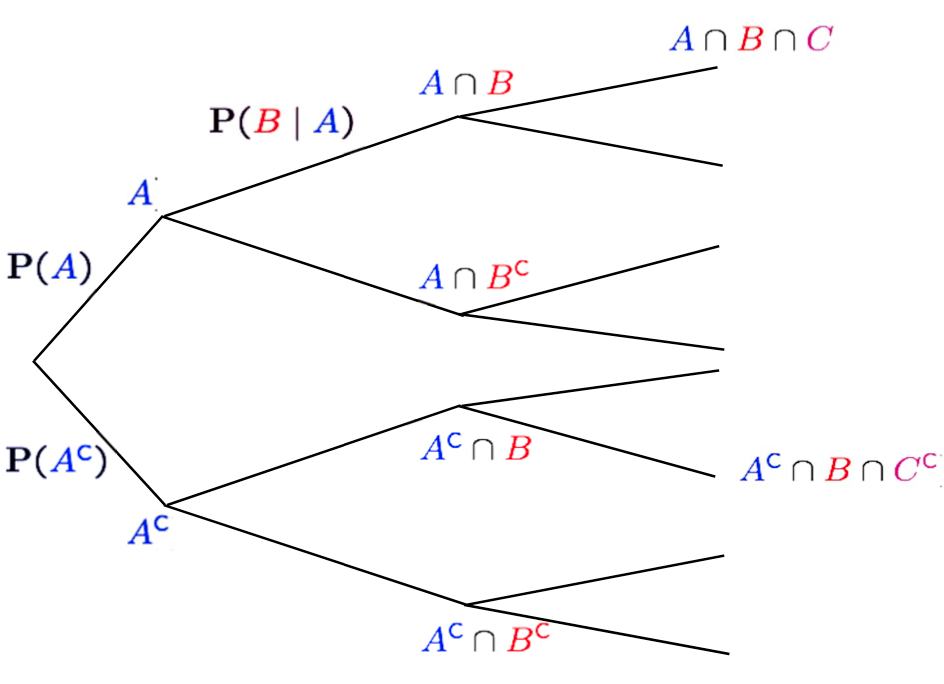
\includegraphics[width=0.85\textwidth]{L2_multi_ex.png}
}

\onslide<6->{
Generally, \hfill \lecturemark{VIDEO PAUSE}

$\cprob{A_1 \cap A_2 \cap \cdots A_n}$ = 
}
\onslide<7->{
$\cprob{A_1} \cdot \cprob{A_2|A_1} \cdot \cprob{A_3|A_1,A_2} \cdots$ $\cprob{A_n|A_1,A_2,\ldots, A_{n-1}}$
}

\end{frame}

%%%%%%%%%%%%%%%%%%%%%%%%%%%%%%%%%%%%%%%%%%%%%%%%%%%%%%
\begin{frame}{Total Probability Theorem}

\footnotetext{Partition: $A_1,A_2,A_3$ are mutually exclusive and $\Omega = A_1 \cup A_2 \cup A_3$}
\mytwocols{0.7}
{
\plitemsep 0.1in
\bci 

\item<1-> \orangef{Partition} of $\Omega$ into $A_1,A_2,A_3$

\item<2-> We know: $\cprob{A_i}$ and $\cprob{B | A_i}$ 

\item<3-> \redf{What is $\cprob{B}$? (probability of result)}

%\bigskip

\begin{block}<4->{Total Probability Theorem}
$$
\cprob{B} = \sum_{i} \cprob{A_i} \cprob{B | A_i}
$$
\end{block}

\item<4-> $\cprob{A_i \cap B} = \cprob{A_i} \cprob{B | A_i}$

\item<5-> Weighted average from the point of $A_i$ knowledge. 
\eci 
}
{
\centering
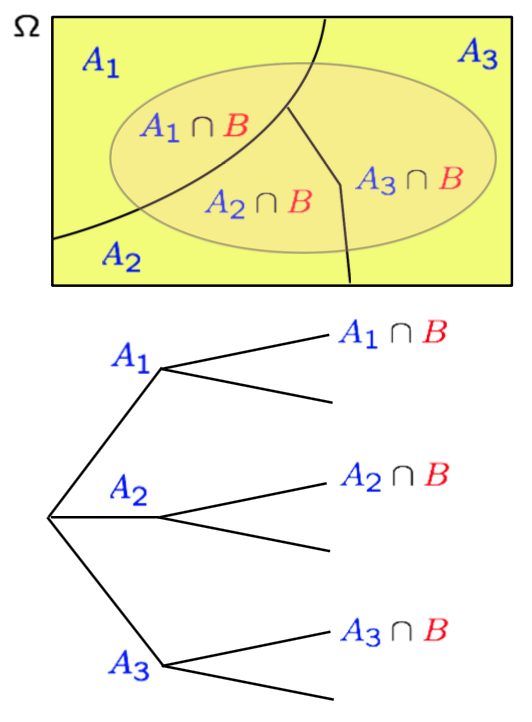
\includegraphics[width=0.65\textwidth]{L2_total_ex.png}
}

\end{frame}

%%%%%%%%%%%%%%%%%%%%%%%%%%%%%%%%%%%%%%%%%%%%%%%%%%%%%%
\begin{frame}{Bayes' Rule}

\mytwocols{0.7}
{
\plitemsep 0.1in

\bci
\item Partition of $\Omega$ into $A_1,A_2,A_3$

\item We know: $\cprob{A_i}$ and $\cprob{B | A_i}$ 

\item<2-> \redf{What is $\cprob{A_i | B}$?}

\item<2-> revised belief about $A_i,$ given $B$ occurs

\begin{block}<3->{Bayes' Rule}
\aleq{
\cprob{A_i | B} &= \frac{\cprob{A_i \cap B}}{\cprob{B}}
 = \frac{\cprob{A_i} \cprob{B | A_i}}{\sum_{j} \cprob{A_j} \cprob{B | A_j}}
}
\end{block}

%\item Weighted average from the point of $A_i$ knowledge. 
\eci 
}
{
\centering
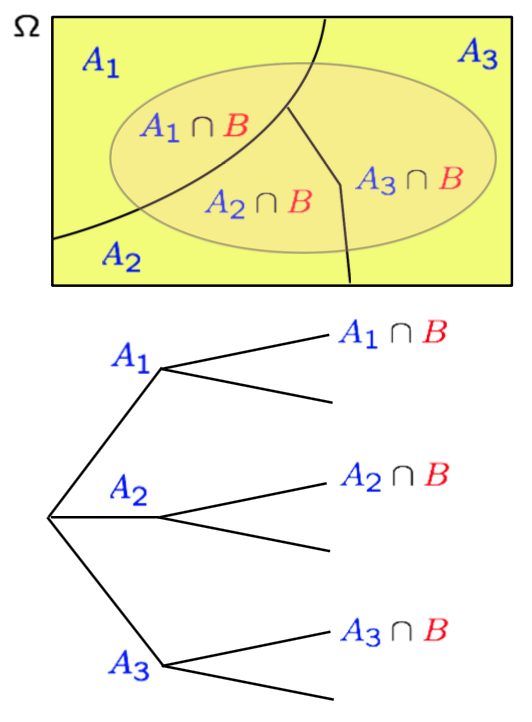
\includegraphics[width=0.65\textwidth]{L2_total_ex.png}
}

\end{frame}

%%%%%%%%%%%%%%%%%%%%%%%%%%%%%%%%%%%%%%%%%%%%%%%%%%%%%%
\begin{frame}{Example 1: Airplane-Radar}

\only<1>{\lecturemark{VIDEO PAUSE}}

\mytwocols{0.7}
{
\plitemsep 0.05in
\bci

\item $A:$ Airplane is flying above 
\item $B:$ Something on radar screen

\eci 

\aleq{
\cprob{A \cap B} &= \onslide<2->{\cprob{A}\cprob{B|A}} \cr
&=\onslide<3->{0.05\times 0.99 = 0.0495}
}
\aleq{
\cprob{B} &= \onslide<4->{\cprob{A \cap B} + \cprob{A^c \cap B}}\cr
&= \onslide<5->{0.05\times 0.99 + 0.95\times 0.1 = 0.1445}
}
\aleq{
\cprob{A|B} &= \onslide<6->{\frac{\cprob{A \cap B}}{\cprob{B}}}
= \onslide<7->{\frac{0.0495}{0.1445} \approx 0.34}
}

% \bigskip
% \item $\cprob{A \cap B} = \cprob{}$
% \bigskip
% \item $\cprob{ B} = $
% \bigskip
% \item $\cprob{A |  B} = $


}
{
\centering

\includegraphics[width=0.5\textwidth]{L2_radar.jpg}

\bigskip
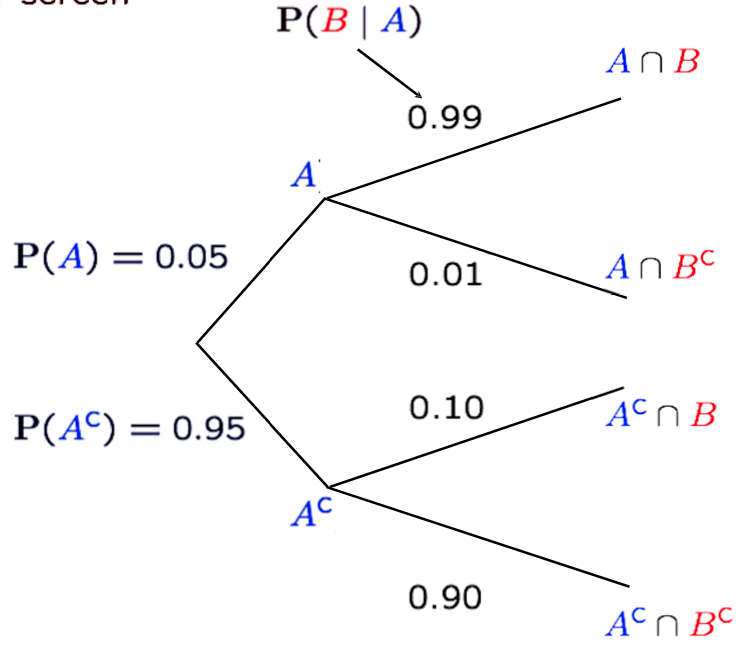
\includegraphics[width=0.7\textwidth]{L2_cond_ex.png}
}
\end{frame}


%%%%%%%%%%%%%%%%%%%%%%%%%%%%%%%%%%%%%%%%%%%%%%%%%%%%%%
\begin{frame}{Example 2: Happy/Sad-Shout}

\mytwocols{0.7}
{
\plitemsep 0.1in
\bci 

\item $A_1$: you are happy, $A_2$: you are sad
\item $B$: you shout. 

\item Assume: 
$$
\cprob{A_1}=0.7, \ \cprob{A_2}=0.3,
$$
$$
\cprob{B | A_1} = 0.3, \ \cprob{B | A_2}=0.5.
$$

\eci 
}
{
\medskip

- Calculate $\cprob{A_1 | B}$ and $\cprob{A_2 | B}.$

\onslide<1>{\hfill \lecturemark{VIDEO PAUSE}}

\onslide<2->{
\aleq{
\cprob{A_1} \cprob{B | A_1} &=  0.7 \times 0.3 = 0.21\cr
\cprob{A_2} \cprob{B | A_2} &= 0.3 \times 0.5 = 0.15 \cr
\cprob{B} &= 0.21 + 0.15 = 0.36
}
\aleq{
\cprob{A_1 | B} = \frac{0.21}{0.36} \approx 0.583 \cr
\cprob{A_2 | B} = \frac{0.15}{0.36} \approx 0.417 
}
}
}

 

\end{frame}


%%%%%%%%%%%%%%%%%%%%%%%%%%%%%%%%%%%%%%%%%%%%%%%%%%%%%%
\section{L2(3)}
\begin{frame}{Roadmap}

\bce[(1)]
\item \grayf{Conditional Probability}

\item \grayf{Bayes' Rule and Bayesian Inference}

\item \redf{Independence, Conditional Independence}

\ece
\end{frame}



%%%%%%%%%%%%%%%%%%%%%%%%%%%%%%%%%%%%%%%%%%%%%%%%%%%%%%
\begin{frame}{}
\vspace{2cm}
\LARGE Bayesian inference was really fun. 

\medskip

Now, let's develop a new concept from conditioning. 

\medskip

\LARGE That is \empr{Independence}. 

\end{frame}

%%%%%%%%%%%%%%%%%%%%%%%%%%%%%%%%%%%%%%%%%%%%%%%%%%%%%%
\begin{frame}{Why We Care Independence?}

\plitemsep 0.1in
\bci 

\item<2-> Event $A$: I get the grade A in the probability class (my interest).
\item<2-> Event $B$: My friend is rich. 

\bigskip
\item<3-> $A$ and $B$ do not seem dependent on each other. So, just forget $B$!

\item<4-> Independence makes our analysis and modeling \redf{much simpler,} because I can remove independent events in the analysis of what I am interested in.  
\eci 
\end{frame}


%%%%%%%%%%%%%%%%%%%%%%%%%%%%%%%%%%%%%%%%%%%%%%%%%%%%%%
\begin{frame}{Independence}

\plitemsep 0.05in
\bci 

\item<1-> Occurrence of $A$ provides \redf{no new information} about $B.$ Thus, knowledge about $A$ does \redf{NOT} change my belief about $B.$ 
$$
\bluef{
\onslide<2->{
\cprob{B | A} = \cprob{B}
}}
$$


\item<3-> Using $\cprob{B | A} = \cprob{B \cap A}/\cprob{A},$ 

\begin{block}<3->{Independence of $A$ and $B$, \redblank{3}{$A \indep B$}}
$\cprob{A \cap B} = \cprob{A} \times \cprob{B}$
\end{block}

\item<4-> The above definition show the \orangef{symmetry} of independence more clearly.

\item<5-> \redf{Q1.} $A$ and $B$ disjoint $\imp$ $A \indep B$?

\onslide<6->{
No. Actually, really dependent, because if you know that $A$ occurred, then, we know that $B$ did not occur. 
}

\item<7-> \redf{Q2.} If $A \indep B$,  then $A \indep B^c$? \onslide<8->{Yes.} 
\eci 
\end{frame}

%%%%%%%%%%%%%%%%%%%%%%%%%%%%%%%%%%%%%%%%%%%%%%%%%%%%%%
\begin{frame}{Conditional Independence}

\plitemsep 0.07in
\bci 

\item<2-> Remember: for a probability law $\cprob{\cdot},$ given some event $C$, $\cprob{\cdot | C}$ is a new probability law. 

\item<3-> Thus, we can talk about independence under $\cprob{\cdot | C}.$

\item<4-> Given that $C$ occurs, occurrence of $A$ provides no new information about $B.$
$$
\bluef{\cprob{B | A \cap C} = \cprob{B | C}}
$$
\vspace{-0.2in}

\item \onslide<6->{Using $\cprob{ A\cap B | C} = \frac{\prob{B \cap (A \cap C)}}{\cprob{C}} = \frac{\cprob{A \cap C}\cprob{B | A\cap C} }{\cprob{C}} = \cprob{A | C} \cprob{B | C},$ }

\begin{block}<5->{Conditional Independence of $A$ and $B$ given $C$, \redblank{5}{$A \indep B | C$}}
$\cprob{A \cap B \redf{| C}} = \cprob{A \redf{|C}} \times \cprob{B \redf{|C}}$
\end{block}



% \smallskip
% \item<7-> \redf{Q1.} If $A \indep B$,  then $A \indep B | C$?
% Suppose that $A$ and $B$ are independent. If you heard that $C$ occurred,  $A$ and $B$ are still independent?                                                         

% \item<8-> \redf{Q2.} If $A \indep B | C$, $A \indep B$?
\eci 
\end{frame}

%%%%%%%%%%%%%%%%%%%%%%%%%%%%%%%%%%%%%%%%%%%%%%%%%%%%%%
\begin{frame}{\redf{(Q1)} $A \indep B$ $\rightarrow$  $A \indep B | C$?}

\plitemsep 0.2in
\bci 

\item Suppose that $A$ and $B$ are independent. If you heard that $C$ occurred,  $A$ and $B$ are still independent? \only<1>{\hfill \lecturemark{VIDEO PAUSE}}

\item<2-> Two independent coin tosses

\plitemsep 0.05in
\bci
\item $H_1$: 1st toss is a head
\item $H_2$: 2nd toss is a head
\item $D$: two tosses have different results.
\eci

\item<3-> $\cprob{H_1 | D} = 1/2,$ $\cprob{H_2 | D} = 1/2$  


\item<4-> $\cprob{H_1 \cap H_2 | D} = 0,$  

\item<5-> No.
\eci 
\end{frame}

%%%%%%%%%%%%%%%%%%%%%%%%%%%%%%%%%%%%%%%%%%%%%%%%%%%%%%
\begin{frame}{\redf{(Q2)} $A \indep B | C$ $\rightarrow$  $A \indep B$?}

\myvartwocols{0.8}{0.7}{0.27}
{
\small
\plitemsep 0.01in
\bci 

% \item \redf{(Q2)} If $A \indep B | C$, $A \indep B$?

\item<2-> Two coins: \bluef{Blue} and \redf{Red}. Choose one uniformly at random, and proceed with two independent tosses. 

\item<3-> $\cprob{\text{head of blue}} = 0.9$ and 
$\cprob{\text{head of red}} = 0.1$ 

$H_i$: i-th toss is head, and $B$: blue is selected. 

\item<4-> $H_1 \indep H_2 | B$? \orangef{Yes}
\aleq{
\cprob{H_1 \cap H_2 | B} = 0.9\times 0.9, \quad \cprob{H_1 |B} \cprob{H_2|B} = 0.9 \times 0.9
}

\item<5-> $H_1 \indep H_2$? \orangef{No}
\abovedisplayskip=-0.01in
\aleq{
\onslide<6->{\cprob{H_1} &= \cprob{B} \cprob{H_1 | B} + \cprob{B^c} \cprob{H_1 | B^c} \cr
&= \frac{1}{2} 0.9 + \frac{1}{2} 0.1 = \frac{1}{2}\cr
\cprob{H_2} &= \cprob{H_1} \quad (\text{because of symmetry})\cr}
\onslide<7->{\cprob{H_1 \cap H_2} &= \cprob{B} \cprob{H_1 \cap H_2| B} + \cprob{B^c} \cprob{H_1 \cap H_2| B^c}\cr 
& = \frac{1}{2} (0.9\times 0.9) + \frac{1}{2} (0.1\times 0.1) \neq \frac{1}{2}}
}
\eci 
}
{
\centering
\onslide<2->{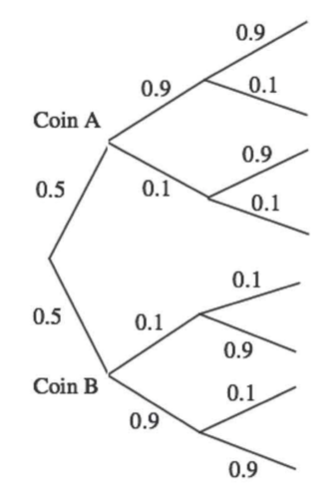
\includegraphics[width=0.8\textwidth]{L2_condind_ex.png}}
}


\end{frame}

%%%%%%%%%%%%%%%%%%%%%%%%%%%%%%%%%%%%%%%%%%%%%%%%%%%%%%
\begin{frame}{Independence of Multiple Events}

\plitemsep 0.1in
\bci 

\item<1-> Three events: $A_1, A_2, A_3.$ What are the conditions of ``their independence"?

\item<2-> What about this? (Pairwise independence)
\begin{align*}
\cprob{A_1 \cap A_2} = \cprob{A_1} \cprob{A_2}, \
\cprob{A_1 \cap A_3} = \cprob{A_1} \cprob{A_3}, \
\cprob{A_2 \cap A_3} = \cprob{A_2} \cprob{A_3}
\end{align*}

\item<3-> What about $\cprob{A_1 \cap A_2 \cap A_3} = \cprob{A_1} \cprob{A_2} \cprob{A_3}$?

\item<4-> We need both. 

\begin{block}<5->{Independence of Multiple Events}
The events $A_1,A_2, \ldots, A_n$ ar said to be independent if
$$
\cbprob{\bigcap_{i \in S} A_i} = \prod_{i \in S} \cprob{A_i}, \quad \text{for every subset } S \text{ of } \{1,2, \ldots, n \}
$$
\end{block}
\eci 
\end{frame}


%%%%%%%%%%%%%%%%%%%%%%%%%%%%%%%%%%%%%%%%%%%%%%%%%%%%%%
\begin{frame}{}
\vspace{2cm}
\LARGE Questions?

\end{frame}

\begin{frame}{Review Questions}
% \tableofcontents
%\plitemsep 0.1in
\bce[1)]
\item What is conditional probability? Why do we need it?

\item Explain the overall framework of Bayesian inference.

\item What is the total probability theorem?

\item What is Bayes' rule? What does it can give us?

\item What's the difference between independence and conditional independence?

\ece
\end{frame}

\end{document}
